\chapter{Projektplanung}

Planung ersetzt den Zufall durch den Irrtum. Albert Einstein \\
Plans are nothing; planning is everything." - Dwight D. Eisenhower \\
"Plane – und du wirst irren. Plane nicht – und du wirst nicht wissen, wo du geirrt hast."
\section{Projekt- und Arbeitsplanung}

\subsection{Kernbestandteile der Projektplanung}
\begin{itemize}
	\item Projektstrukturplan - Aufteilung in Themenblöcke: \\ 
	- Phasenorientiert: Anforderungerhebung, Architektur \& Design, Implementation \\
	- Objektorientiert: Benutzerschnittstelle, Datenhaltung, Anwendungsfunktionalität, Kommunikation, Systemdienste \\
	- nach Verantwortung: QS, Fortschrittskontrolle, Anwendungs- und/oder Nutzungsfälle (Use Cases)
	\item Arbeitspakete \\
	beschreiben eine klar definierte Tätigkeit, definierte Dauer, zugeordnete Ressourcen sowie (logische oder zeitliche) Abhängigkeiten von anderen Arbeitspaketen 
	\item Zeit-/Terminplan (ggf. nur die nächsten Arbeitspakete "ausdetailieren")
	\item Meilensteinplan \\
	- Feststellen der Zielerreichung \\
	- Kann erfüllt oder nicht erfüllt sein \\
	- Blockierende Meilensteine (z.B. Projekt nicht genehmigt - Projekt steht still)\\
	-  Meilensteine sollten nicht zu nahe zusammenliegen)
	\item Schätzungen (siehe VL 7 Aufwandsschätzung)
\end{itemize}

Der Inhalt von Arbeitspaketen umfasst einen eindeutigen Identifikator, einen Namen zur Bezeichnung, eine Beschreibung des Arbeitspakets, Verantwortliche und mitwirkende Rollen/Personen, die geschätzte Dauer des Arbeitspakets, Ergebnisdefinition (geforderte Artefakte), Qualitätsanforderungen, Abnahmekriterien, technische Abhängigkeiten sowie zu erfassende Kennzahlen


\begin{figure}[ht]
	\centering
	\adjustbox{width=11cm}{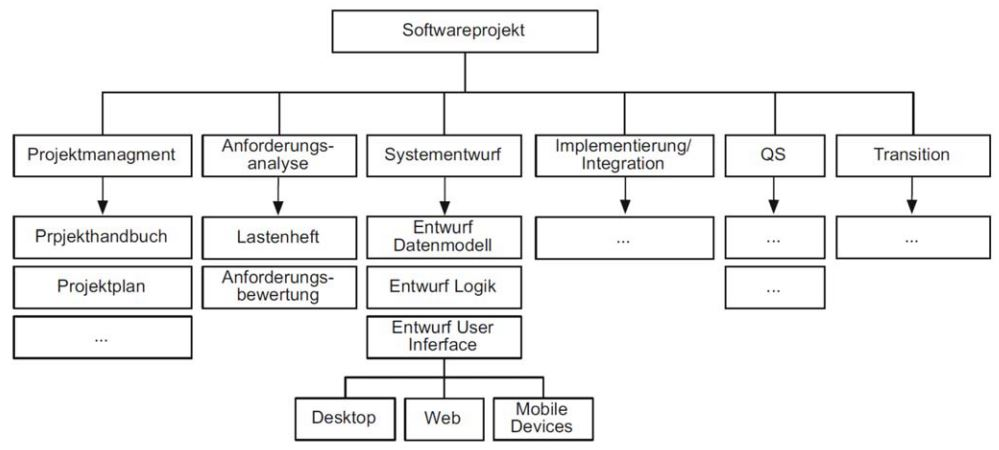
\includegraphics{Figures/Projektstrukturplan}}
	\caption[]{Projektstrukturplan}
\end{figure}

\begin{figure}[ht]
	\centering
	\adjustbox{width=11cm}{\includegraphics{Figures/Meilensteinplan}}
	\caption[]{Meilensteinplan}
\end{figure}

\subsection{Netzplantechnik}
 Grafische Darstellung der Zeitpunkte für die Durchführung von Tätigkeiten \\
 Logische Beziehungen und zeitliche Anordnung zwischen den Arbeitspaketen wird dargestellt. \\
Wie lange wird das Projekt (mindestens) dauern?
Welche kritischen Arbeitspakete können das gesamte Projekt verzögern?

\textbf{Methoden}
\begin{multicols}{2}
\begin{itemize}
	\item Critical Path Method
	\item Program Evaluation Review Technique (PERT)
	\item Meta Potential Method (MPM)  
\end{itemize}
\columnbreak

	\adjustbox{width=4cm}{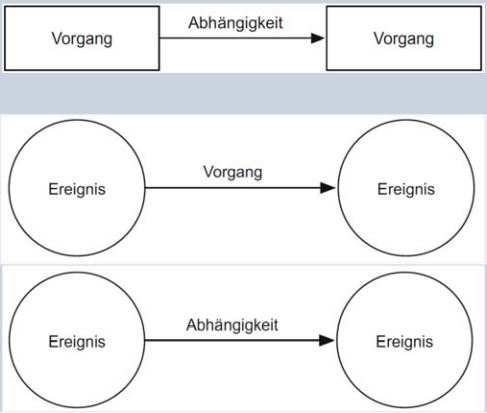
\includegraphics{Figures/npmethoden}}

\end{multicols}

\textbf{Modellierung} \\
Kritischer Pfad berechnen:
Wie in Digitaltechnik - Zeiten berechnen für ein Signal im Netzwerk.
Verkettung von derjenigen Vorgänge, bei 
deren zeitlicher Änderung sich der 
Endtermin des Netzplanes verschiebt. Aktivität a liegt auf einem kritischen Pfad bei p(a) = 0. Falls es keinen Projekt-Endtermin gibt hat man mindestens einen kritischen Pfad.

Vorwärtsrechnung: \\
Frühster Endtermin fet(a): Frühster Anfangstermin fat(a) + Vorgangsdauer d(a)

Rückwärtsrechnung: \\
Spätester Anfangstermin sat(a) = spätester Endtermin set(a) - Vorgangsdauer d(a)

Puffer: \\
Zeitdauer in der man die Aktivität herum schieben kann, ohne, dass sich das Projekt verzögert.
\\ Puffer p(a) = spätester Endtermin set(a) - frühster Endtermin fet(a) \\
 = spätester Anfangstermin sat(a) - frühster Anfangstermin fat(a)

\subsection{Balkenplantechnik - Gantt-Diagramm}

\begin{minipage}{7.5cm}
	Normalfolge: End-Anfang-Beziehung \\
	B startet wenn A fertig ist
\end{minipage}
\begin{minipage}{7.4cm}
	Anfangsfolge: Anfang-Anfang-Beziehung \\
	A und B müssen zeitgleich starten
\end{minipage}

\adjustbox{width=7.5cm}{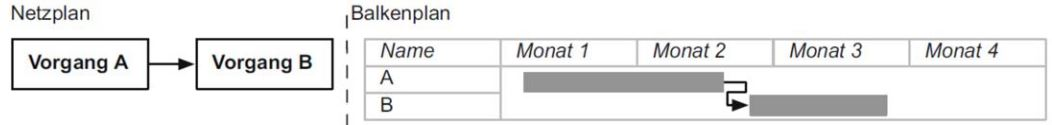
\includegraphics{Figures/normalfolge}}
\adjustbox{width=7.4cm}{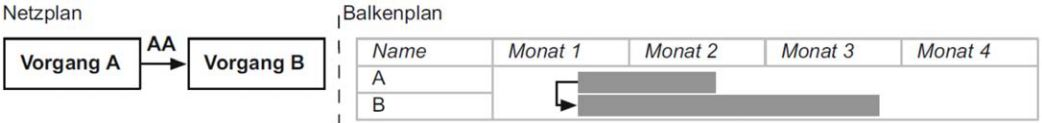
\includegraphics{Figures/anfangsfolge}}


\begin{minipage}{7.5cm}
	Endfolge: End-End-Beziehung \\
	A und B müssen zeitgleich beendet werden
\end{minipage}
\begin{minipage}{7.4cm}
	Sprungfolge: Anfang-End-Beziehung \\
	B kann erst beendet werden, wenn A anfängt
\end{minipage}

\adjustbox{width=7.5cm}{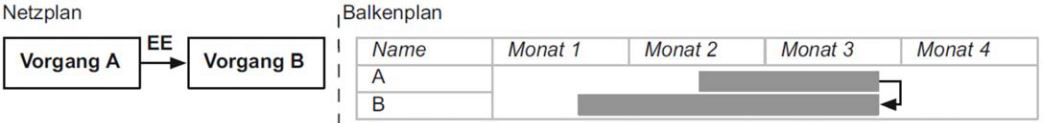
\includegraphics{Figures/endfolge}}
\adjustbox{width=7.4cm}{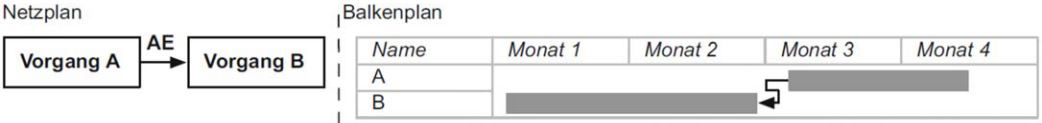
\includegraphics{Figures/sprungfolge}}

\subsubsection{Projektplanung in der Praxis}
- Netzpläne: für Grobplanung und prozessorientierte Darstellung \\
- Arbeitspakete werden oft zu stark unterteilt, Arbeitspakete mit Dauer < 1 Woche sollten ggf. überdacht werden \\
- Keine Abhängigkeiten zwischen Arbeitspaketen, wo keine notwendig sind: \\
--> Zuerst Pflichtenheft erstellen, dann Design / Implementation (Abhängigkeit) \\
--> Implementation und Test können parallel gemacht werden (keine Abhängigkeit) \\
--> Lieber eine Abhängigkeit weniger machen

Es gibt verschiedene Philosophien zur Projektplanung. Darunter sind Meilenstein-orientierte Planung, Fast Tracking, Time Boxing, Critical Chain und Kanban.




